\documentclass{scrreprt}
\usepackage{graphicx}
\graphicspath{ {images/} }
\usepackage{listings}
\usepackage{underscore}
\usepackage[bookmarks=true]{hyperref}
\usepackage{hyperref}
\usepackage{graphicx}
\usepackage[english]{babel}
\usepackage[utf8]{inputenc}
\usepackage{float}
\pagenumbering{arabic}
\usepackage{fancyhdr}
\fancypagestyle{plain}{
	\fancyhf{}% Clear header/footer
	\fancyhead[L]{Software Metrics Calculation System User Manual}% Left header
	\fancyfoot[C]{\thepage}
}

\hypersetup{
	bookmarks=false,    % show bookmarks bar?
	pdftitle={Software Metrics Calculation System User Manual},    % title
	pdfauthor={Christopher Silva},                     % author
	pdfsubject={TeX and LaTeX},                        % subject of the document
	pdfkeywords={TeX, LaTeX, graphics, images}, % list of keywords
	colorlinks=true,       % false: boxed links; true: colored links
	linkcolor=blue,       % color of internal links
	citecolor=black,       % color of links to bibliography
	filecolor=black,        % color of file links
	urlcolor=purple,        % color of external links
	linktoc=page            % only page is linked
}%
\author{Christopher Silva}
\date{}
\def\myversion{1.0 }
\begin{document}
	\begin{titlepage}
		\flushright
		\LARGE{ID-10-T}
		
\includegraphics[scale=0.08]{logo.png}
		\rule{16cm}{5pt}\vskip1cm
		\centering
		\Huge{Software Metrics Calculation System}\\
		\vspace{2cm}
		\Huge{Test plan}\\
		\vspace{2cm}
		\LARGE{Version \myversion\\}
		\vspace{2cm}
		Prepared by\\
	    Christopher Silva\\
	    Shujing Zhang\\
		Anthony Enem\\
		Nathan Durst\\
		Da Dong\\
		\vfill
		\rule{16cm}{5pt}
	\end{titlepage}
	\pagenumbering{roman}
	\tableofcontents
%============================================================================
	\chapter{Introduction}
	\pagenumbering{arabic}
	
	\section{Test Purpose}
	This document describes the plan for testing the Software Metrics Calculation System (SMCS) . This Test Plan document supports the following objectives:
	Identify the required resources and provide an estimate of the test efforts.
	List the deliverable elements of the test activities.
	Recommend and describe the testing strategies to be employed.

	\section{Product Overview}
	The main objective of SMCS is to help first and second year computer science students become better programmers.
	This software will calculate and display metrics about the users source code such as line of code, lines of documentation, cyclical complexity, etc.
	These metrics will be used to give the user feedback on their code and to correct commonly made mistakes.
	
	\section{Scope}
	This is a List of test type we are going to follow
	\begin{itemize}
		\item Test 1: Unit Testing 
		\item Test 2: validation Testing 
		\item Test 3: System Testing
	\end{itemize}
	
%============================================================================
	{\let\clearpage\relax \chapter{Testing Requirement}}
	
	\section{Hardware Requirements}
	

	\section{Software Requirements}
	Operating System: Windows XP, OS X 10.7, Linux 2.6.23\\
	Web Browser: Firefox, Chrome, Edge, Safari\\

%============================================================================
	{\let\clearpage\relax \chapter{Getting Started}}
	\section{How to Start SMCS}
	To start SMCS in standalone mode simply double click on the application. 
	This will start a local web server on port 8080 and launch your default web browser to the SMCS code submission page. 
	If you wish to host SMCS on a server so that it is accessible from anywhere, open config.json and change the "standalone" configuration option to false, ensure that port 8080 is forwarded correctly and then start SMCS. 
	SMCS will only open the web browser if it is in standalone mode.

	\section{User interface}
	The user interface is split into two pages, a source code submission page, and an analysis results page. The next three pages show these two pages labeled with descriptions of the UI elements.
	
	\begin{figure}[H]
		\centering
		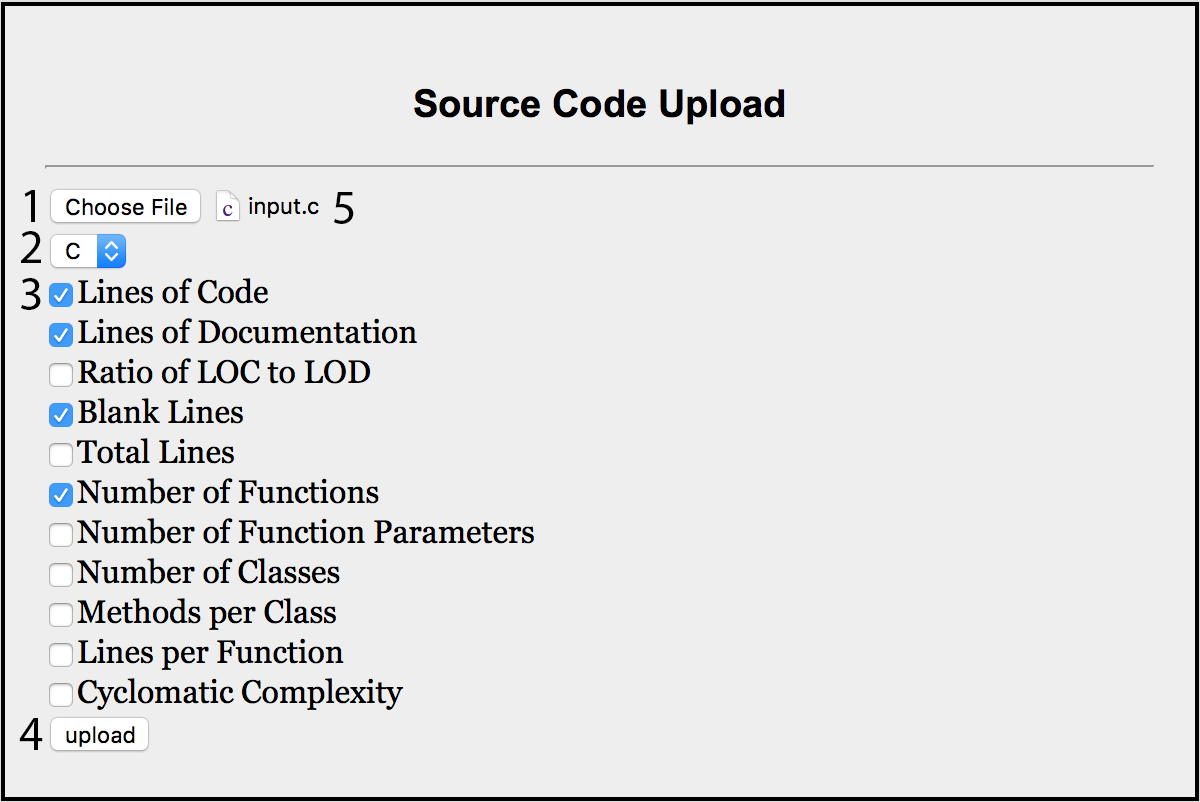
\includegraphics[scale=0.7]{lguiu.png}
		\caption{Source Code Submission page with labeled elements}
	\end{figure}
	
	This page is used to select the source code and metrics you want to use in the analysis.
	
	\begin{enumerate}
		\item Choose File - Use this button to select a source code file.
		\item Language Selection - If the correct language is not automatically selected, use this combobox to select the correct one.
		\item Metrics Selection - Use these checkboxes to select the metrics you wish to use.
		\item Upload - Use this button to run the selected metrics on your source code.
		\item File Name - This is the file that is currently selected.
	\end{enumerate}
	
	\begin{figure}[H]
		\centering
		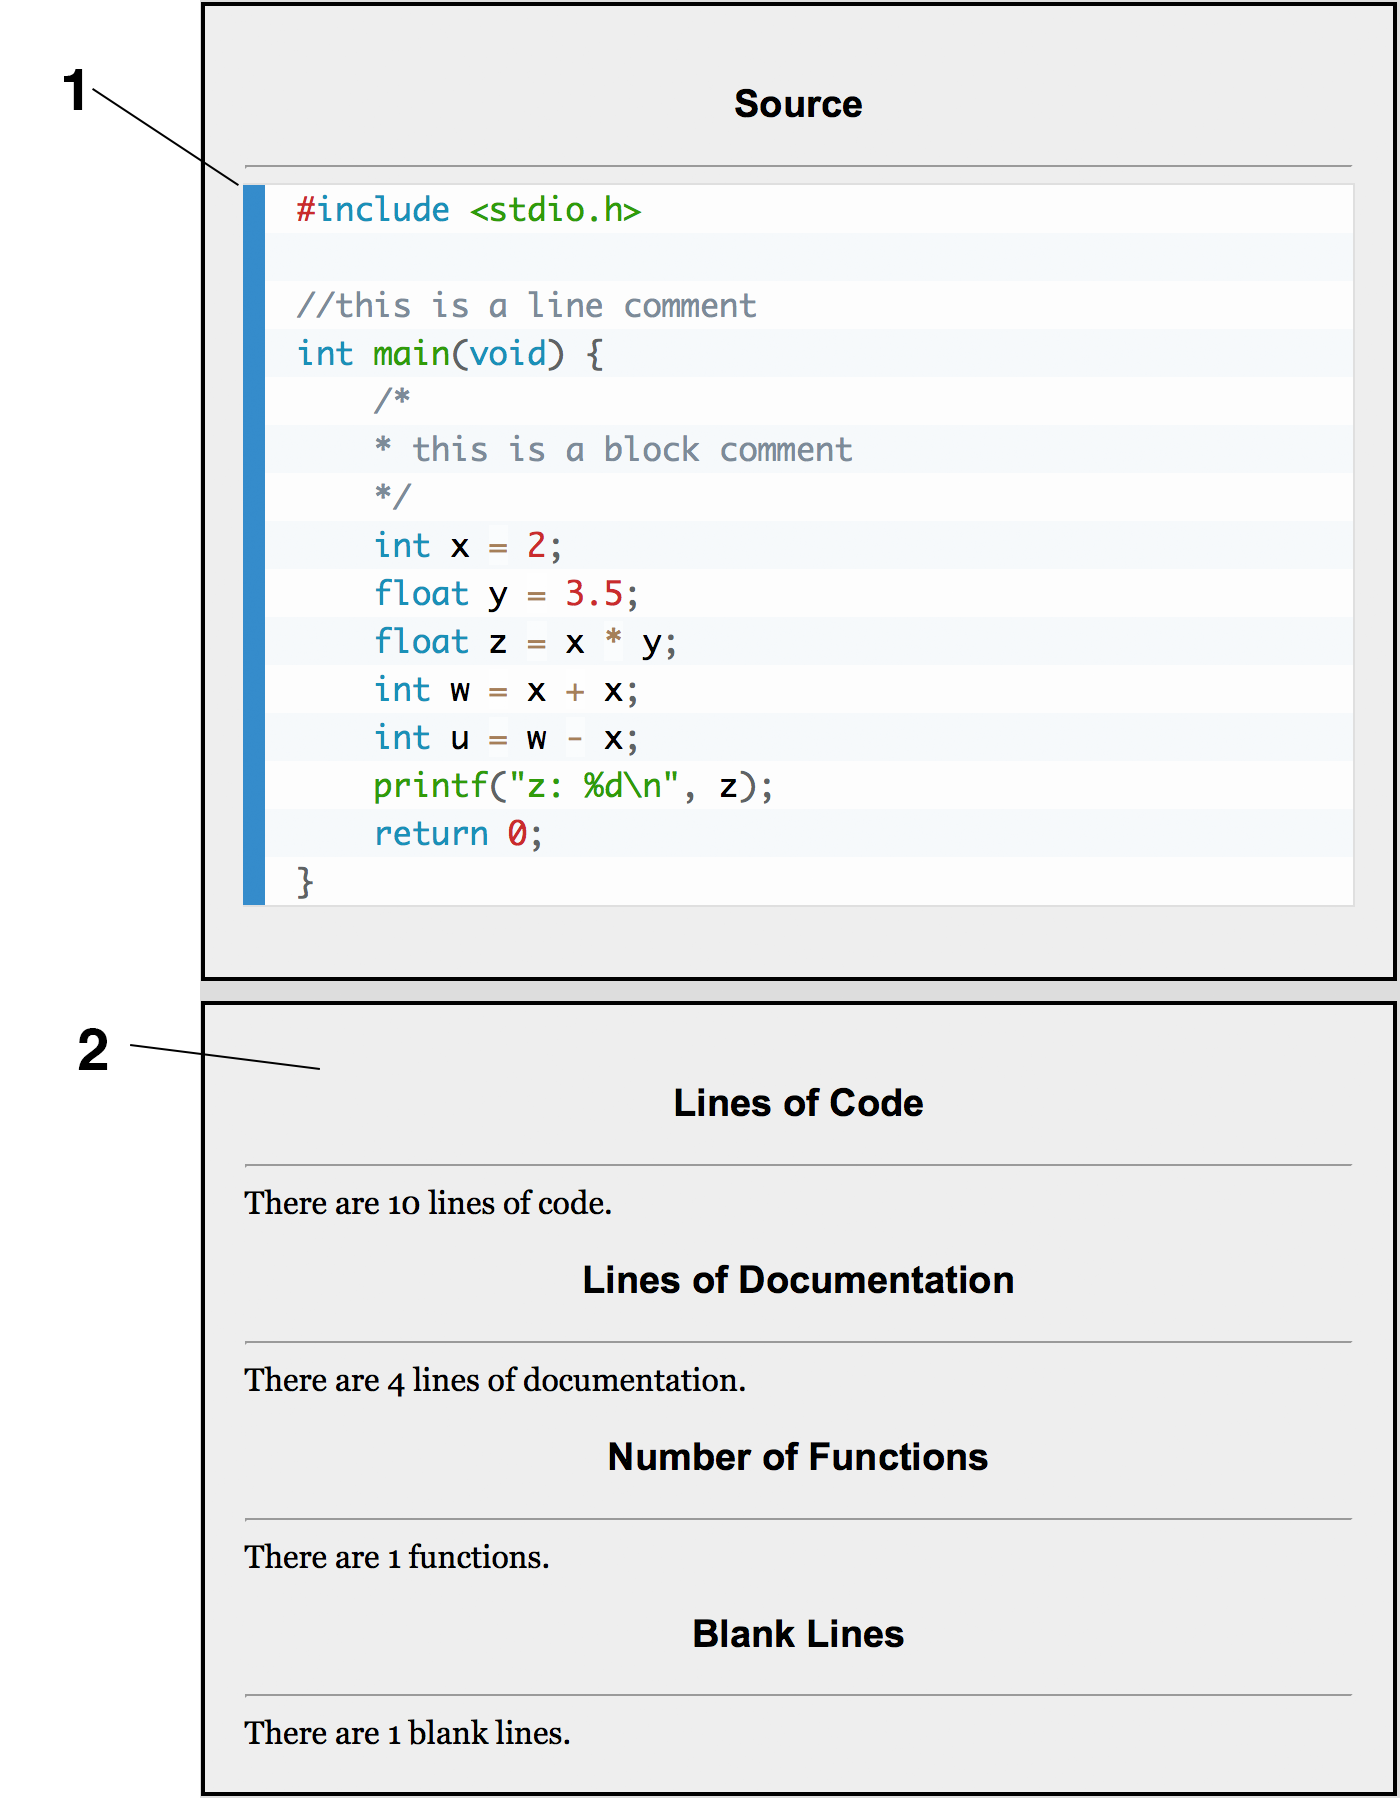
\includegraphics[scale=0.7]{lguir.png}
		\caption{Analysis Results page with labeled elements}
	\end{figure}
	
	This page shows your selected source code and the results of the analysis.
	
	\begin{enumerate}
		\item Source Code - Your selected source code file syntax highlighted
		\item Metrics Results - A listing of the results of the metrics you selected.
	\end{enumerate}
	

%============================================================================
	{\let\clearpage\relax \chapter{Available Metrics}}
	This chapter describes the metrics available to use in SMCS.
	
	\section{Lines of ...}
	\begin{itemize}
		\item Code - The number of lines of code in your source.
		\item Documentation - The number of lines of documentation in your source.
		\item Ratio - The ration of Lines of Code to Lines of Documentation. It could be a problem if the ratio of documentation to code is too low.
		\item Whitespace - The number of blank lines in you source.
		\item Total Lines - The total number of lines in your source.
	\end{itemize}
	Note: A line that contains code and documentation will be counted as both a line of code and documentation.
	
	\section{Number of ...}
	\begin{itemize}
		\item Functions - The number of functions in your source.
		\item Function parameters - The number of parameters in each function. If you have too many parameters in a function it could cause trouble, especially if it is used often.
		\item Classes - The number of 
		\item Methods per Class - The number of methods in each class.
		\item Lines per Function - the number of lines in each function.
	\end{itemize}
	
	\section{Cyclomatic Complexity}
	Cyclomatic Complexity is the number of linearly independent paths within a program. \\
	It is used to measure the complexity of a program. \\
	
	Example C code:
	\begin{lstlisting}
	if (A == 10) {
	    if (B > C) {
	        A = B;
	    } else {
	        A = C;
	    }
	}
	printf(A);
	printf(B);
	printf(C);
	\end{lstlisting}
	This code has a three  separate paths that it can take so it has a cyclomatic complexity of three. 

%============================================================================	
	{\let\clearpage\relax \chapter{Appendix}}
	
	\section{How to Report a Bug}
	If you find any bugs, please tell us by sending an email to ID10T.BUG@example.com\\
	Please include the following information when reporting a bug:\\
	\begin{itemize}
		\item A complete description of the problem what led to it.
		\item What operating system and web browser you are using.
		\item What error messages are displayed.
	\end{itemize}
	
	\section{Contacts}
		Contact information for ID-10-T team members.\\
		\begin{tabular}{|l|c|}
			\hline
			Member Name       & Phone Number \\ \hline
			Christopher Silva & 940-782-1234 \\ \hline
			Anthony Enem      & 940-782-2345 \\ \hline
			Nathan Durst      & 940-782-3456 \\ \hline
			Da Dong           & 940-782-4567 \\ \hline
			Shujing Zhang     & 940-782-6789 \\ \hline
		\end{tabular}
\end{document}
